\chapter{Dispositif expérimental}


Afin de pouvoir réaliser les mesures présentées dans cette thèse, il a fallu réunir au sein d’un même dispositif expérimental, une électronique temps réel, un convertisseur courant tension bas bruit, un réfrigérateur a dilution ainsi qu’un système magnétique permettant de balayer le champ magnétique a des vitesses relativement élevées, de l’ordre de plusieurs dizaines de Tesla par seconde. Le schéma correspondant est présenté dans la Fig.\ref{ann3fig}. Nous allons détailler chacun des éléments de cette structure.

\section{Automate de mesure : ADwin}
Afin de pouvoir réaliser un transistor moléculaire, nous avons vu, dans le chapitre second, qu’il était nécessaire de procéder a une électromigration. Afin que cette dernière se passe dans de bonnes conditions, il faut être capable de contrôler la tension appliquée à la jonction, et ce, dans un délai de l’ordre
de quelques microsecondes. Or, lorsqu’une mesure est acquise à l’aide d’un ordinateur, comme cela est habituellement le cas, ce délai ne peut pas être garanti du fait du caractère multitâche des systèmes d’exploitation. Un moyen de s’affranchir de cette limitation est d’avoir recours à un automate.

\begin{figure}
\centering 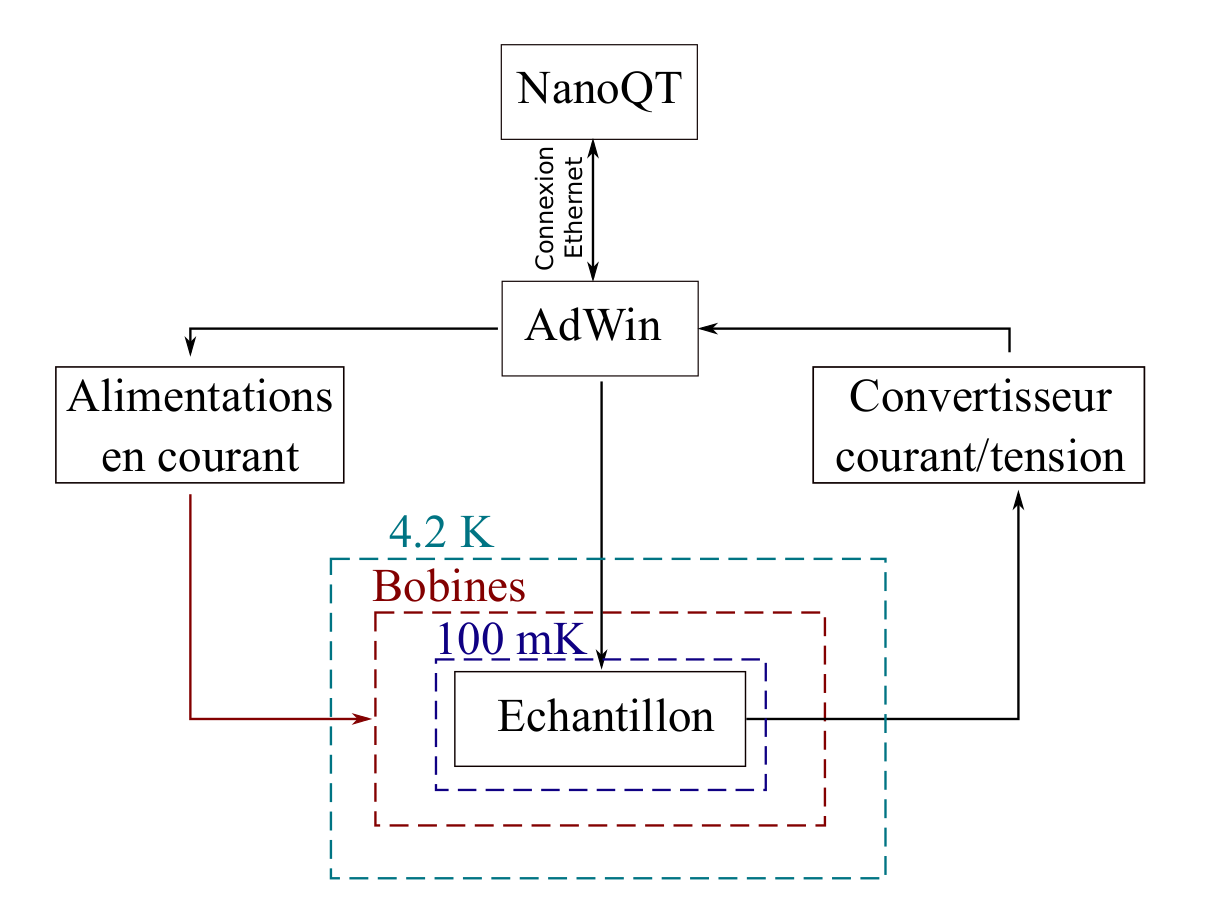
\includegraphics[scale=0.35]{Annexe4/annexe4fig.png}
\caption{Diagramme de notre dispositif expérimental. L’automate AdWin est commandé à l’aide du logiciel NanoQt à travers la rédaction de scripts. Cet automate prend en charge les commandes relatives aux bobines, à la polarisation de l’échantillon ainsi qu’à l’acquisition des données qui sont renvoyées vers l’ordinateur pour traitement . Un réfrigérateur à dilution permet de refroidir l’échantillon à une température électronique de 100 mK. Les bobines, immergées dans l’hélium liquide, sont à une température de 4.2 K.}
\label{ann3fig}
\end{figure}

Ce dernier va exécuter une série d’instructions dans un temps bien défini, ce qui permet de connaître de façon précise le temps de réponse dans le cas de boucles de contre-réaction. Et c’est justement sur une boucle de contre réaction qu’est basée notre technique d’électromigration. Celle-ci permet de ramener la tension aux bornes de la jonction à zéro lorsque la conductance de cette dernière passe en dessous d’une valeur seuil. En ce qui concerne notre équipe, nous avons décidé d’utiliser un automate de type ADwin. Celui-ci peut être programmé à l’aide d’un langage propriétaire, le ADbasic, afin d’effectuer des opérations dans un timing précis. Il dispose de huit entrées et autant de sorties, pouvant être contrôlées séparément, et qui permettent notamment de polariser nos échantillons en tension, mais également de contrôler la valeur et la direction du champ magnétique comme nous le verrons dans la section suivante. La programmation de l’automate a principalement été réalisée par Edgard Bonet aidé de Raoul Piquerel et de Christophe Thirion. A l’aide de ce programme, l’automate est capable de contrôler et de commander ses entrées et sorties toutes les 10$\mu$s soit la durée minimale pour un bon contrôle de l’électromigration.

\section{Le logiciel de commande : NanoQT}
Cependant, la diversité des mesures que nous avons présentées peut difficilement être rendue compatible avec l’utilisation d’un automate, car pour chaque procédure il faudrait le reprogrammer. C’est pour cela qu’un jeu d’instructions simples compose le programme exécuté par l’automate lui même. Pour permettre d’effectuer des mesures complexes, il a fallu mettre au point un protocole ainsi qu’une interface afin de pouvoir envoyer, de façon asynchrone, les différentes instructions relatives a une mesure. Encore une fois, Edgard, Raoul et Christophe se sont attelés à la tâche et ont développé un programme nommé NanoQT (prononcer ”nano cute” en référence à la librairie graphique QT). Ce dernier permet, par l’intermédiaire de scripts en JavaScript, non seulement de mettre au point des protocoles de mesure complexes, mais également de tracer, traiter (au moins en partie) et sauvegarder ces dernières.


Les instructions sont envoyées à l’automate par une connexion Ethernet également utilisée pour récupérer les données. Le script le plus simple se compose d’une instruction de balayage. Cette dernière comprend notamment le
chemin à parcourir dans l’espace des paramètres expérimentaux, en général : la tension source drain V$_{ds}$ , la tension de grille V$_g$ et le champ magnétique. Sont également précisés les paramètres de la détection synchrone, lorsque cela est nécessaire, ainsi que les paramètres à mesurer et à tracer et/ou sauvegarder. A partir d’une instruction de balayage, il est ensuite possible d’établir des procédures de mesure complexes tout en ayant l’assurance que le timing décidé est bien celui exécuté lors de la mesure.

\section{Convertisseur courant-tension}
Le développement des convertisseurs que j’ai utilisés durant ma thèse a été réalisé par Daniel Lepoittevin et Nicolas Roch, le doctorant m’ayant précédé (et formé). La difficulté principale est de réaliser, dans un même
dispositif, une amplification bas bruit pour les mesures en transport, mais également une amplification faible gain et grande bande passante, permettant la mesure et le contrôle de l’électromigration. Différents modèles ont été développés et je renvoie le lecteur curieux è la thèse de Nicolas Roch pour plus d’information [54].


\section{Système magnétique}
Afin de réaliser des mesures sur le retournement de l’aimantation d’une manière efficace, il est nécessaire de balayer le champ magnétique relativement vite, dans notre cas, de l’ordre de quelques dizaines de milli Telsas par seconde. De plus, il faut pouvoir choisir un vecteur magnétique dans les trois dimensions de l’espace.

Lorsque je suis arrivé en thèse, nous ne disposions que d’une bobine à forte inductance qui, certes, nous donnait accès a des champs magnétiques élevés, mais n’autorisait pas une vitesse de balayage supérieure è quelques
dixièmes de milli Telsa par seconde, du fait notamment d’un effet de chauffe trop important induit par les courants de Foucault. De plus, celle-ci ne permettait de balayer le champ que dans une seule direction, n’autorisant pas, par exemple, l’identification éventuelle de l’axe d’anisotropie d’un aimant moléculaire comme cela a été montré dans le chapitre trois de cette thèse. 

Nous avons donc décidé de fabriquer, en collaboration avec Eric Eyraud, un ensemble de deux bobines de faible taille, l’une ayant une géométrie standard, la seconde étant de type Helmoltz. Ce changement nous a également
obligés à modifier le porte-échantillon, et à mettre au point un système de doigt très fin, sur lequel repose notre échantillon et qui vient se glisser au centre des deux bobines composant l’ensemble.

Après quelques simulations, les deux bobines ont été réalisées par Eric Eyraud afin de permettre un champ selon l’axe z de 4.5 T pour 115 ampères et un champ de 1.8 T selon l’axe z pour un courant de 120 ampères. La vitesse
de balayage maximale de notre système et d’environ 100 mT par seconde, une vitesse supérieure entraînant une hausse de la température de notre système. Le troisième axe est obtenu par rotation du frigo à dilution, l’axe de rotation étant l’axe $z$.

Le courant est délivré par deux alimentations de courant de type Boutnik pouvant fournir jusqu’à 120 ampères et atteindre une vitesse de rampe de plus de 10 ampères par seconde. Afin d’être synchronisées avec le reste de la mesure, les deux alimentations sont contrôlées par l’automate par l’intermédiaire d’une tension. Ceci permet de parfaitement corréler la valeur du champ avec la conductance mesurée lors des différents protocoles.

